\documentclass[12pt,a4paper]{article}

% The report is designed for Tectonic's XeTeX engine and Overleaf.
\usepackage{fontspec}
\setmainfont{Liberation Serif}
\setmonofont{Liberation Mono}[Scale=MatchLowercase]
\usepackage[english]{babel}
\usepackage[left=2cm,right=1.5cm,top=2cm,bottom=2cm]{geometry}
\usepackage{setspace}
\usepackage{graphicx}
\usepackage{xcolor}
\usepackage{listings}
\usepackage{fancyvrb}
\usepackage{titlesec}
\usepackage{caption}
\usepackage{float}
\usepackage{array}
\usepackage{booktabs}
\usepackage[hidelinks]{hyperref}

\graphicspath{{figures/}}
\onehalfspacing
\setlength{\parindent}{1.25cm}
\setlength{\parskip}{0pt}
\setlength{\emergencystretch}{2em}

% All numbers of the text come from the csv files (made by plots/make_figures.py).
% generated by plots/make_figures.py - do not edit
\newcommand{\aMsOne}{440}
\newcommand{\aSpeedOne}{1.00}
\newcommand{\aMemOne}{28.0}
\newcommand{\aPoolMsOne}{440}
\newcommand{\aPoolSpeedOne}{1.00}
\newcommand{\aMsTwo}{230}
\newcommand{\aSpeedTwo}{1.92}
\newcommand{\aMemTwo}{28.9}
\newcommand{\aPoolMsTwo}{234}
\newcommand{\aPoolSpeedTwo}{1.88}
\newcommand{\aMsFour}{123}
\newcommand{\aSpeedFour}{3.59}
\newcommand{\aMemFour}{30.1}
\newcommand{\aPoolMsFour}{125}
\newcommand{\aPoolSpeedFour}{3.51}
\newcommand{\aMsEight}{68}
\newcommand{\aSpeedEight}{6.51}
\newcommand{\aMemEight}{34.1}
\newcommand{\aPoolMsEight}{70}
\newcommand{\aPoolSpeedEight}{6.28}
\newcommand{\aMsSixteen}{74}
\newcommand{\aSpeedSixteen}{5.97}
\newcommand{\aMemSixteen}{42.4}
\newcommand{\aPoolMsSixteen}{72}
\newcommand{\aPoolSpeedSixteen}{6.09}
\newcommand{\aMsThirtyTwo}{69}
\newcommand{\aSpeedThirtyTwo}{6.41}
\newcommand{\aMemThirtyTwo}{58.9}
\newcommand{\aPoolMsThirtyTwo}{68}
\newcommand{\aPoolSpeedThirtyTwo}{6.51}
\newcommand{\aMsSixtyFour}{72}
\newcommand{\aSpeedSixtyFour}{6.13}
\newcommand{\aMemSixtyFour}{88.2}
\newcommand{\aPoolMsSixtyFour}{71}
\newcommand{\aPoolSpeedSixtyFour}{6.20}
\newcommand{\aSecOne}{0.440}
\newcommand{\aSecBest}{0.068}
\newcommand{\aSpeedBest}{6.51}
\newcommand{\aGainSMT}{-8}
\newcommand{\aPoolMaxDiff}{3}
\newcommand{\aRunsEach}{5}
\newcommand{\aMemExtraPerThread}{1.0}
\newcommand{\bThreads}{16}
\newcommand{\bRuns}{9}
\newcommand{\bNoSyncMsMin}{239}
\newcommand{\bNoSyncMsMax}{636}
\newcommand{\bNoSyncMs}{337}
\newcommand{\bLockMs}{3059}
\newcommand{\bLockMsMin}{2382}
\newcommand{\bLockMsMax}{4939}
\newcommand{\bPerThreadMs}{21}
\newcommand{\bPerThreadMsMin}{17}
\newcommand{\bPerThreadMsMax}{22}
\newcommand{\bNoSyncRatio}{16}
\newcommand{\bLockRatio}{147}
\newcommand{\bLockOverNoSync}{9}
\newcommand{\bNoSyncCountMin}{6.2}
\newcommand{\bNoSyncCountMax}{9.6}
\newcommand{\bNoSyncShareMax}{19}
\newcommand{\bMemMin}{234}
\newcommand{\bMemMax}{236}
\newcommand{\cSecOne}{1.24}
\newcommand{\cSpeedOne}{1.00}
\newcommand{\cMemOne}{206}
\newcommand{\cPoolSecOne}{1.31}
\newcommand{\cPoolMemOne}{206}
\newcommand{\cSecTwo}{1.23}
\newcommand{\cSpeedTwo}{1.01}
\newcommand{\cMemTwo}{102}
\newcommand{\cPoolSecTwo}{1.15}
\newcommand{\cPoolMemTwo}{94}
\newcommand{\cSecFour}{1.26}
\newcommand{\cSpeedFour}{0.98}
\newcommand{\cMemFour}{93}
\newcommand{\cPoolSecFour}{1.26}
\newcommand{\cPoolMemFour}{102}
\newcommand{\cSecEight}{1.29}
\newcommand{\cSpeedEight}{0.96}
\newcommand{\cMemEight}{144}
\newcommand{\cPoolSecEight}{1.34}
\newcommand{\cPoolMemEight}{140}
\newcommand{\cSecSixteen}{1.28}
\newcommand{\cSpeedSixteen}{0.97}
\newcommand{\cMemSixteen}{185}
\newcommand{\cPoolSecSixteen}{1.29}
\newcommand{\cPoolMemSixteen}{182}
\newcommand{\cSecThirtyTwo}{1.38}
\newcommand{\cSpeedThirtyTwo}{0.90}
\newcommand{\cMemThirtyTwo}{266}
\newcommand{\cPoolSecThirtyTwo}{1.29}
\newcommand{\cPoolMemThirtyTwo}{182}
\newcommand{\cSecSixtyFour}{1.58}
\newcommand{\cSpeedSixtyFour}{0.79}
\newcommand{\cMemSixtyFour}{338}
\newcommand{\cPoolSecSixtyFour}{1.30}
\newcommand{\cPoolMemSixtyFour}{206}
\newcommand{\cBestWorkers}{2}
\newcommand{\cSecBest}{1.23}
\newcommand{\cSpeedBest}{1.01}
\newcommand{\cOverAOne}{2.8}
\newcommand{\cOverABest}{18}
\newcommand{\cSlowdownSixtyFour}{27}
\newcommand{\cPoolGainSixtyFour}{18}
\newcommand{\cPoolMemSavedSixtyFour}{133}
\newcommand{\cOneMin}{1.13}
\newcommand{\cOneMax}{1.40}
\newcommand{\tUsbSecOne}{17.19}
\newcommand{\tUsbSpeedOne}{1.00}
\newcommand{\tUsbReadOne}{16.4}
\newcommand{\tUsbParseOne}{0.75}
\newcommand{\tUsbMemOne}{72}
\newcommand{\tUsbSpreadOne}{0.4}
\newcommand{\tSsdMsOne}{497}
\newcommand{\tSsdSpeedOne}{1.00}
\newcommand{\tUsbSecTwo}{17.64}
\newcommand{\tUsbSpeedTwo}{0.97}
\newcommand{\tUsbReadTwo}{34.5}
\newcommand{\tUsbParseTwo}{0.75}
\newcommand{\tUsbMemTwo}{116}
\newcommand{\tUsbSpreadTwo}{0.3}
\newcommand{\tSsdMsTwo}{279}
\newcommand{\tSsdSpeedTwo}{1.78}
\newcommand{\tUsbSecFour}{18.60}
\newcommand{\tUsbSpeedFour}{0.92}
\newcommand{\tUsbReadFour}{71.9}
\newcommand{\tUsbParseFour}{0.74}
\newcommand{\tUsbMemFour}{205}
\newcommand{\tUsbSpreadFour}{0.1}
\newcommand{\tSsdMsFour}{210}
\newcommand{\tSsdSpeedFour}{2.37}
\newcommand{\tUsbReadShare}{96}
\newcommand{\tUsbOverA}{39}
\newcommand{\tUsbOverSsd}{35}
\newcommand{\tUsbMiBs}{21}
\newcommand{\tSsdReadShare}{15}
\newcommand{\tSsdParseOne}{0.42}
\newcommand{\tSsdReadOne}{0.07}


\definecolor{codebackground}{HTML}{F3F4F6}
\definecolor{codeframe}{HTML}{D1D5DB}
\definecolor{commentgreen}{HTML}{3F6212}
\definecolor{keywordblue}{HTML}{1D4ED8}
\definecolor{outputbackground}{HTML}{111827}
\definecolor{outputtext}{HTML}{F9FAFB}

\titleformat{\section}
  {\normalfont\bfseries\centering\fontsize{13}{16}\selectfont}
  {\thesection}{0.8em}{\MakeUppercase}
\titleformat{name=\section,numberless}
  {\normalfont\bfseries\centering\fontsize{13}{16}\selectfont}
  {}{0pt}{\MakeUppercase}
\titleformat{\subsection}
  {\normalfont\bfseries\fontsize{12}{15}\selectfont}
  {\thesubsection}{0.7em}{}
\titlespacing*{\section}{0pt}{0pt}{12pt}
\titlespacing*{\subsection}{0pt}{10pt}{6pt}

\lstdefinestyle{csharp}{
  language=[Sharp]C,
  basicstyle=\ttfamily\footnotesize,
  keywordstyle=\color{keywordblue}\bfseries,
  commentstyle=\color{commentgreen},
  backgroundcolor=\color{codebackground},
  frame=single,
  rulecolor=\color{codeframe},
  breaklines=true,
  columns=fullflexible,
  keepspaces=true,
  showstringspaces=false,
  numbers=left,
  numberstyle=\tiny\color{gray},
  escapeinside={(*@}{@*)},
  xleftmargin=0.5cm,
  framexleftmargin=0.4cm,
  aboveskip=7pt,
  belowskip=7pt
}

\DefineVerbatimEnvironment{terminaloutput}{Verbatim}{
  fontsize=\footnotesize,
  frame=single,
  framesep=3mm,
  rulecolor=\color{codeframe}
}

\begin{document}

% -----------------------------------------------------------------------------
% Title page
% -----------------------------------------------------------------------------
\begin{titlepage}
  \begin{center}
    \IfFileExists{figures/LOGO_UTM.jpg}{%
      
\includegraphics[width=3.4cm]{figures/LOGO_UTM.jpg}\par
      \vspace{0.25cm}
    }{}

    {\bfseries\fontsize{14}{17}\selectfont
      MINISTRY OF EDUCATION AND RESEARCH\par
      OF THE REPUBLIC OF MOLDOVA\par
      Technical University of Moldova\par
      Faculty of Computers, Informatics and Microelectronics\par
      Department of Software Engineering and Automation\par
    }

    \vspace{0.8cm}
    {\bfseries\fontsize{16}{19}\selectfont
      Moisei Daniel, FAF-241\par
      Strulea Teodor, FAF-242\par}

    \vspace{0.8cm}
    {\bfseries\fontsize{36}{40}\selectfont Report\par}
    \vspace{0.25cm}
    {\itshape\fontsize{20}{24}\selectfont Laboratory Work No. 1\par}
    {\bfseries\itshape\fontsize{20}{24}\selectfont Network Programming (PR)\par}

    \vspace{0.7cm}
    {\fontsize{20}{25}\selectfont Topic: Concurrency in Practice\par}
    \vspace{0.2cm}
    {\fontsize{15}{19}\selectfont CPU-bound and I/O-bound Work, Race Conditions, Speed-up\par}
  \end{center}

  \vfill
  \begin{flushright}
    {\fontsize{15}{18}\selectfont Checked by:}\par
    \textbf{Fi\c{s}tic Cristofor}, \textit{assistant lecturer}
  \end{flushright}

  \vfill
  \begin{center}
    {\bfseries\fontsize{14}{17}\selectfont Chi\c{s}in\u{a}u -- 2026}
  \end{center}
\end{titlepage}

\pagenumbering{arabic}
\setcounter{page}{2}
\tableofcontents
\newpage

\section*{Introduction}
\addcontentsline{toc}{section}{Introduction}

The purpose of this laboratory work is to measure how the number of threads, and the way the work is divided among them, change the running time and the memory of a real workload: counting the negative, zero and positive integers of a text file with 50\,000\,000 numbers. From the measurements we decide when the work is CPU-bound and when it is I/O-bound, observe a race condition and the price of removing it, and find where the parallel speed-up stops.

The work was done jointly by Moisei Daniel (FAF-241) and Strulea Teodor (FAF-242). The program is written in C\# (.NET 10) and follows the style of the lectures: threads are created with \texttt{new Thread}, every thread writes only into its own slot of an array, shared counters are protected by \texttt{lock (gate)}, and the producer and the consumers use a blocking queue. Every task is one class that implements the interface \texttt{ITask}, and the task and its settings are chosen on the command line. In addition to the tasks of the assignment, we compared our own threads with threads taken from the thread pool (Tasks~1a and~1c). Every run appends one row to a csv file (\texttt{task1a\_results.csv}, \dots), and all tables, charts and numbers of this report are produced from these files by a script.

\newpage
\section{Short Theory}

\subsection{CPU-bound and I/O-bound Work}

A program is \textit{CPU-bound} when its speed is limited by the processor: it keeps the processor busy, and more cores make it faster. It is \textit{I/O-bound} when it spends most of its time waiting for input and output, for example for a file on a disk or a USB drive, or for the network; then the processor is mostly idle and the speed is limited by the device.

\subsection{Cores, Logical Processors and Speed-up}

A physical core is a complete computing unit. With hyper-threading the core has two ``inboxes'' and the operating system sees two logical processors; when one task waits (for data from memory, for example), the core switches to the other. In practice the gain is 15--30\%, and a program that already keeps the core fully busy gains almost nothing. If $T(p)$ is the time with $p$ threads, the speed-up is
\begin{equation}
  S(p)=\frac{T(1)}{T(p)}.
\end{equation}

\subsection{Race Conditions}

The statement \texttt{counter++} is three operations: read, add, write. A thread can be stopped between any two of them, so two threads that increment the same variable can overwrite each other's result. A race needs shared mutable state and more than one thread; the fixes of the lecture remove one of them: do not share (a slot or a variable for each thread), or make the access exclusive with \texttt{lock}.

\subsection{Thread Pool}

With \texttt{new Thread} we own the thread and pay for creating it. With \texttt{Task.Run} or \texttt{ThreadPool.\allowbreak QueueUserWorkItem} we submit work and the runtime owns the threads: it keeps a limited number of them and reuses them. The rule of the lecture is never to block a pool thread, because while it waits it serves nobody. On this machine the pool starts with as many threads as logical processors (16) and adds more only slowly.

\section{Environment and Measurement Method}

\subsection{Hardware and Software}

Table~\ref{tab:hardware} describes the machine. The data was collected with \texttt{lscpu}, \texttt{free}, \texttt{lsblk} and \texttt{lsusb -t}; the raw output is saved in \texttt{data/hardware.txt}. The USB version was read from the kernel (\texttt{/sys/bus/usb/devices}): the drive declares USB~2.00 and is attached at 480~Mbit/s, although the laptop also has 10~Gbit/s ports.

\begin{table}[H]
  \centering
  \caption{Hardware and software}
  \renewcommand{\arraystretch}{1.25}
  \begin{tabular}{>{\raggedright\arraybackslash}p{0.27\textwidth}>{\raggedright\arraybackslash}p{0.6\textwidth}}
    \toprule
    \textbf{Item} & \textbf{Value} \\
    \midrule
    Processor & AMD Ryzen 7 6800HS, up to 4.79~GHz \\
    Cores and threads & 8 physical cores, 16 logical processors (2 threads per core), L2 4~MiB, L3 16~MiB \\
    Memory & 14~GiB RAM \\
    Internal disk & Micron 2450 NVMe SSD, 954~GB \\
    USB drive & ``General USB Flash Disk'' (ID \texttt{ffff:5678}), 29.3~GB, ext4; USB~2.0, 480~Mbit/s \\
    Operating system & CachyOS, Linux 7.3.0-4-cachyos, x86-64 \\
    Language and runtime & C\# on .NET 10.0.13 (SDK 10.0.113), Release build \\
    \bottomrule
  \end{tabular}
  \label{tab:hardware}
\end{table}

\subsection{Input and Correctness}

\texttt{numbers.txt} contains 50\,000\,000 random integers in $[-1\,000\,000,\,1\,000\,000]$, one per line, produced by \texttt{System.Random} with seed 12345; the file has 369\,454\,226 bytes (352.3~MiB). The command \texttt{generate} counts the numbers while it writes them, so the correct answer is known:

\begin{center}
  \renewcommand{\arraystretch}{1.15}
  \begin{tabular}{lr}
    \toprule
    Negative & 25\,007\,776 \\
    Zero & 22 \\
    Positive & 24\,992\,202 \\
    \midrule
    Total & 50\,000\,000 \\
    \bottomrule
  \end{tabular}
\end{center}

For Task~2 the command \texttt{split} cuts the file, in order, into eight files of 6\,250\,000 numbers. Every task prints the three counters and checks that they add up to 50\,000\,000. In the tables of this report all runs found exactly the counters above; the only exception is the unsynchronised version of Task~1b, which is wrong by design.

\subsection{Timing, Memory and Aggregation}

Every measurement is a separate process, so the peak memory belongs to that run only. The time is taken with a \texttt{Stopwatch} and includes opening the file, creating the threads, counting, waiting for the threads and adding the partial results; it does not include the start of the runtime, and in Task~1b it does not include loading the array. The peak memory is the peak working set of the process (\texttt{PeakWorkingSet64}).

Tasks~1a and~1c were run \aRunsEach{} times for every number of threads (own threads and thread pool alternately, after two warm-up runs, so the file was in the page cache and the results do not show the speed of a cold disk). Task~1b was run in three separate processes, each with three runs of version 1 (\bRuns{} runs of version 1 in total), and Task~2 three times for every number of threads. The tables give the median (for Task~2 the mean of three runs); the charts also show every run and the minimum--maximum range. The laptop was also running a desktop session, so differences of a few per cent between neighbouring configurations are within the noise.

\newpage
\section{Implementation}

\subsection{Program Structure}

Every task is a class that implements the interface \texttt{ITask} with the single method \texttt{Run(string[] args)}, and contains all its logic, including the creation of its threads. \texttt{Program.cs} only chooses the class from the first command-line argument. The files are: \texttt{GenerateTask}, \texttt{SplitTask}, \texttt{Task1a}, \texttt{Task1b}, \texttt{Task1c}, \texttt{Task2}, \texttt{Counts} (the counters and the parser), \texttt{Args} (reading \texttt{--threads 8}) and \texttt{Results} (peak memory and the csv files).

\begin{lstlisting}[style=csharp,caption={Choosing the task in Program.cs}]
ITask? task = args[0] switch
{
    "generate" => new GenerateTask(),
    "split" => new SplitTask(),
    "task1a" => new Task1a(),
    "task1b" => new Task1b(),
    "task1c" => new Task1c(),
    "task2" => new Task2(),
    _ => null
};
\end{lstlisting}

\subsection{Parsing Without Strings}

The numbers of Tasks~1a and~2 are parsed directly from the bytes of the file in one pass: the digits are accumulated into an integer, a minus sign is remembered, and at every newline the number is counted. No string is created. The method returns how many bytes it used; the unfinished last line of a buffer is carried to the next block.

\begin{lstlisting}[style=csharp,caption={The parser of Counts.cs}]
for (int i = 0; i < text.Length; i++)
{
    byte b = text[i];

    if (b >= '0' && b <= '9')
    {
        number = number * 10 + (b - '0');
        hasDigits = true;
    }
    else if (b == '-')
    {
        minus = true;
    }
    else if (b == '\n')
    {
        if (hasDigits) Add(minus ? -number : number);
        number = 0;
        minus = false;
        hasDigits = false;
        used = i + 1;
    }
}
\end{lstlisting}

\subsection{Task 1a: Dividing the File Without Splitting a Line}

Cutting the file at $\mathit{size}\cdot i/N$ would usually stop in the middle of a line. The start of part $i$ is therefore the first byte after the first newline found at or after the byte \emph{before} the cut; if that byte is itself a newline, the line begins exactly at the cut and is not skipped. Each thread asks for its own start and for the start of the next part, which is its end. The same position always gives the same answer, so a line belongs to exactly one thread. Each thread reads its part in blocks of 1~MiB with positional reads (\texttt{RandomAccess.Read}) and never reads the whole file.

\begin{lstlisting}[style=csharp,caption={Start of a part (Task1a.cs)}]
long position = size * index / partCount - 1;
byte[] buffer = new byte[4096];

while (position < size)
{
    int read = RandomAccess.Read(file, buffer, position);
    if (read == 0) break;

    int newLine = Array.IndexOf(buffer, (byte)'\n', 0, read);
    if (newLine >= 0)
        return position + newLine + 1;

    position += read;
}
return size;
\end{lstlisting}

The threads are created as in the lectures; the option \texttt{--pool} replaces them with tasks of the thread pool. Both versions write into their own element of the array \texttt{counts}, which is summed after the threads have finished.

\begin{lstlisting}[style=csharp,caption={Own threads and thread pool in Task1a.cs}]
if (usePool)
{
    Task[] tasks = new Task[threadCount];
    for (int i = 0; i < threadCount; i++)
    {
        int index = i;
        tasks[i] = Task.Run(() => { counts[index] = CountPart(file, size, index, threadCount); });
    }
    Task.WaitAll(tasks);
}
else
{
    Thread[] threads = new Thread[threadCount];
    for (int i = 0; i < threadCount; i++)
    {
        int index = i;
        threads[i] = new Thread(() => { counts[index] = CountPart(file, size, index, threadCount); });
        threads[i].Start();
    }
    foreach (Thread thread in threads)
        thread.Join();
}
\end{lstlisting}

\subsection{Task 1b: Shared Counters}

The numbers are first loaded into an \texttt{int[]} (not measured), then the array is cut into equal ranges, one for each thread. The three versions differ only in the loop. In the first the threads increment shared counters without any protection, in the second every update is inside \texttt{lock (gate)}, in the third every thread counts in its own variable and the results are added after \texttt{Join}.

\begin{lstlisting}[style=csharp,caption={Version 2, shared counters under a lock (Task1b.cs)}]
long[] shared = new long[3];
object gate = new object();
...
for (int k = from; k < to; k++)
{
    lock (gate)
    {
        if (numbers[k] < 0) shared[0]++;
        else if (numbers[k] == 0) shared[1]++;
        else shared[2]++;
    }
}
\end{lstlisting}

\begin{lstlisting}[style=csharp,caption={Version 3, a counter for each thread (Task1b.cs)}]
Counts mine = new Counts();   // only this thread uses it
for (int k = from; k < to; k++)
    mine.Add(numbers[k]);
counts[index] = mine;
\end{lstlisting}

\subsection{Task 1c: Producer and Consumers}

One reader thread reads the file line by line, collects 10\,000 lines in a \texttt{List<string>} and puts it into a \texttt{BlockingCollection} with the capacity of 100 batches. \texttt{Add} waits while the queue is full; \texttt{GetConsumingEnumerable} waits while it is empty and ends after the reader has called \texttt{CompleteAdding}. Every worker counts into its own slot of an array.

\begin{lstlisting}[style=csharp,caption={Reader and workers of Task1c.cs}]
string? line;
while ((line = reader.ReadLine()) != null)
{
    batch.Add(line);
    if (batch.Count == BatchSize)
    {
        queue.Add(batch);   // waits here while the queue is full
        batch = new List<string>(BatchSize);
    }
}

if (batch.Count > 0)
    queue.Add(batch);

queue.CompleteAdding();   // no more batches: the workers can stop
...
// waits while the queue is empty, ends after CompleteAdding when nothing is left
foreach (List<string> batch in queue.GetConsumingEnumerable())
{
    foreach (string line in batch)
        counts.Add(int.Parse(line));
}
\end{lstlisting}

\subsection{Task 2: Files on the USB Drive}

The eight files are divided in contiguous blocks among the threads (8, 4 or 2 files for a thread with 1, 2 or 4 threads). A thread reads a whole file with one operation into one byte buffer, parses the buffer, and uses the same buffer for its next file. The time of the reading and the time of the parsing are measured separately, which is what shows whether the work is I/O-bound.

\begin{lstlisting}[style=csharp,caption={Reading and parsing a file in Task2.cs}]
using (FileStream stream = File.OpenRead(files[k]))
{
    length = (int)stream.Length;
    stream.ReadExactly(buffer, 0, length);   // the whole file at once
}
long afterRead = Stopwatch.GetTimestamp();

counts[index].AddText(buffer.AsSpan(0, length), true);
long afterParse = Stopwatch.GetTimestamp();
\end{lstlisting}

\subsection{Tools Used and Why}

For every task we used the simplest tool that does what the assignment asks; the alternatives from the lectures that were not used are named, with the reason.

\textbf{All tasks.} \texttt{Thread} with \texttt{Start} and \texttt{Join}, as in lecture 1: the assignment asks for threads created by the program. \texttt{Join} is enough to wait, because every task has one phase, so a \texttt{Barrier} (which waits for all workers at the end of each phase) is not needed. Every thread writes only into its own element of an array (\texttt{Counts[]}): this is the first step of the ladder in lecture 2, \textit{don't share}, so there is no race, and the array is summed after \texttt{Join}. The time is measured with \texttt{Stopwatch}, a monotonic clock (\texttt{DateTime.Now} can jump), and the peak memory is \texttt{PeakWorkingSet64}, the highest amount of RAM the process has used; each measurement is a new process, so earlier runs do not count.

\textbf{Task 1a.} The threads read with \texttt{RandomAccess.Read(handle, buffer, offset)}. It reads at a given position and does not use or change a common file position, so all threads can share one open file without a lock. With one \texttt{FileStream} the threads would share one position (\texttt{Seek} followed by \texttt{Read} from two threads is a race), and one stream for each thread would work but opens the file many times. A buffer of 1~MiB for each thread keeps the memory small: a thread never holds more than one block. The experiment with the thread pool uses \texttt{Task.Run}: we submit work and the runtime owns the threads.

\textbf{Task 1b.} \texttt{lock (gate)}, where \texttt{gate} is a private object used only for this purpose, as the lecture asks (step 4). \texttt{Interlocked} (step 3) is another correct way for one variable, but the assignment asks for exactly three versions: no synchronisation, a lock or mutex, and a counter for each thread (step 1). \texttt{Mutex} is a heavier operating-system object meant to be shared between processes; \texttt{lock} is the light in-process mutex of C\#. The loading of the array (not measured) uses \texttt{File.ReadLines} and \texttt{int.Parse}, which is the simplest way and does not keep 50 million strings in memory at once, as \texttt{ReadAllLines} would.

\textbf{Task 1c.} \texttt{BlockingCollection} with a capacity of 100 batches gives, in one object, everything the assignment describes. \texttt{Add} waits while the queue is full (the reader waits); \texttt{GetConsuming\allowbreak Enumerable} waits while it is empty (the workers wait); \texttt{CompleteAdding} closes the queue, and the loops of the workers end by themselves when it is empty, so no special ``end'' item is needed. These are the \textit{Add} and \textit{Take} of the producer--consumer picture of lecture 3. The alternatives:
\begin{itemize}
  \item \texttt{SemaphoreSlim} limits \emph{how many} threads are inside, or counts free places, but it carries no data (lecture 2). A bounded queue would need two semaphores (free places and filled places), a lock around an ordinary queue, and a way to tell the workers that the file has ended. \texttt{BlockingCollection} does all of this with less room for mistakes. A semaphore is the right tool to allow, for example, at most three downloads at a time.
  \item \texttt{ConcurrentQueue} is thread-safe but never blocks and has no limit. The workers would have to wait for items by busy waiting (a whole core burns) or by sleeping in a loop (they wake up late), the two bad ways of waiting in lecture 3, and the queue could grow without limit.
  \item \texttt{Channel<T>} can also be bounded, but its reading and writing are made for \texttt{async}/\texttt{await}. Our reader and workers are threads that compute, and blocking on an async method with \texttt{.Result} breaks rule 1 of lecture 3; \texttt{async} makes waiting cheap and does not make computing faster.
  \item An own queue with \texttt{lock} and \texttt{Monitor.Wait}/\texttt{Pulse} is allowed by the assignment, but it is more code and it is easy to lose a wake-up.
\end{itemize}
A batch is a \texttt{List<string>} of 10\,000 lines, so the lock of the queue is taken once for 10\,000 lines. The reader uses \texttt{StreamReader.ReadLine}, because the assignment says that it reads line by line.

\textbf{Task 2.} A file is read with \texttt{File.OpenRead} and \texttt{ReadExactly}: one call that fills one \texttt{byte[]} with the whole file (not a list of lines), repeating the read internally if the system returns fewer bytes. \texttt{File.ReadAllBytes} would also read a file at once, but it allocates a new array of about 46~MB for every file; with one buffer for each thread, reused for its next file, the peak memory is about the number of threads times the size of a file (\tUsbMemOne{}, \tUsbMemTwo{} and \tUsbMemFour{}~MB in Table~\ref{tab:task2}). \texttt{Stopwatch.GetTimestamp} is taken before and after the reading and the parsing, to separate the two times. The files are divided in advance, in blocks: 8 equal files divide evenly among 1, 2 and 4 threads, so a queue would only add a lock and give nothing (control question~\ref{cq:queue}).

\newpage
\section{Task 1: Counting One File}

\subsection{Task 1a: Counting with Threads}

Figure~\ref{fig:task1a} and Table~\ref{tab:task1a} show the run with 1 to 64 threads; the blue line is the program with its own threads (the answer to the assignment), the orange line is the same program with tasks of the thread pool (Section~\ref{sec:pool}).

\begin{figure}[H]
\centering
\caption{Task 1a: execution time, speed-up and peak memory}
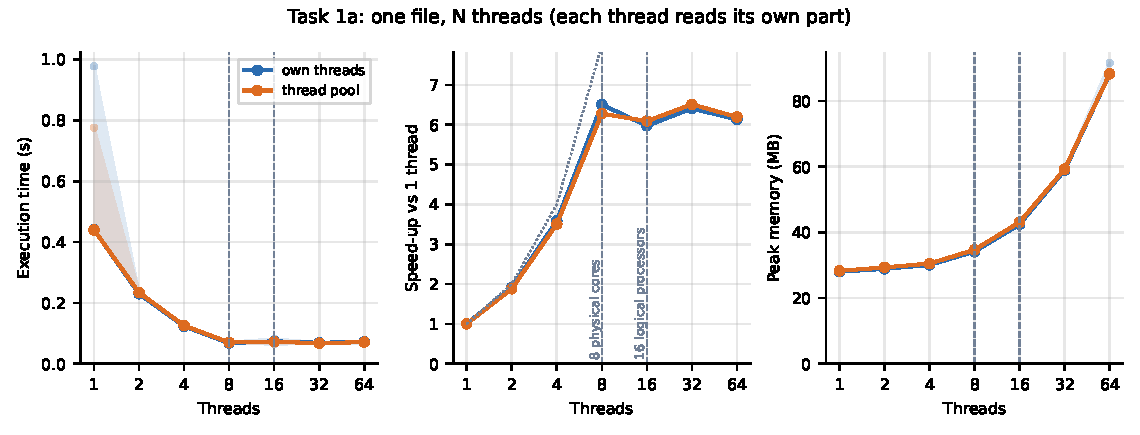
\includegraphics[width=\textwidth]{task1a.pdf}
\label{fig:task1a}
\end{figure}

\begin{table}[H]
  \centering
  \caption{Task 1a, median of \aRunsEach{} runs; the last three columns are the thread-pool variant}
  \resizebox{\textwidth}{!}{\begin{tabular}{rrrrrrr}
\toprule
Threads & Time (ms) & Speed-up & Peak mem. (MB) & Pool: time (ms) & Pool: speed-up & Pool: peak mem. (MB) \\
\midrule
1 & 440 & 1.00 & 28.0 & 440 & 1.00 & 28.3 \\
2 & 230 & 1.92 & 28.9 & 234 & 1.88 & 29.3 \\
4 & 123 & 3.59 & 30.1 & 125 & 3.51 & 30.5 \\
8 & 68 & 6.51 & 34.1 & 70 & 6.28 & 34.7 \\
16 & 74 & 5.97 & 42.4 & 72 & 6.09 & 43.1 \\
32 & 69 & 6.41 & 58.9 & 68 & 6.51 & 59.2 \\
64 & 72 & 6.13 & 88.2 & 71 & 6.20 & 88.2 \\
\bottomrule
\end{tabular}
}
  \label{tab:task1a}
\end{table}

\textbf{1. At which number of threads does the speed-up stop growing? Relate it to the physical cores and the logical processors.} The speed-up is close to ideal up to four threads (\aSpeedTwo{} with two, \aSpeedFour{} with four) and reaches \aSpeedEight{} with eight threads, the number of physical cores: the time falls from \aMsOne{}~ms to \aMsEight{}~ms. After that it does not grow: with 16 threads, the number of logical processors, the speed-up is \aSpeedSixteen{}, and with 32 and 64 threads \aSpeedThirtyTwo{} and \aSpeedSixtyFour{}, all within the noise of the run-to-run variation. Hyper-threading therefore gave nothing here. This agrees with the lecture: the second logical processor only fills the moments in which a core waits, and our loop that parses the bytes keeps the core fully busy. That eight threads give 6.5 and not 8 times the speed is probably due to the memory and to the file cache that all threads share; we did not measure it.

\textbf{2. Why do 32 and 64 threads not help? Are they slower?} They are not slower: \aMsThirtyTwo{}~ms and \aMsSixtyFour{}~ms against \aMsEight{}--\aMsSixteen{}~ms for 8 and 16 threads. They do not help because the machine has only 16 logical processors: the additional threads wait for a time slice, and the work is already finished in about 70~ms, so there is nothing left to share.

\textbf{3. Does the peak memory depend on the number of threads? Why?} Yes. It grows from \aMemOne{}~MB with one thread to \aMemSixtyFour{}~MB with 64, about \aMemExtraPerThread{}~MB for every thread. The file is never loaded as a whole: each thread has a read buffer of 1~MiB (and a stack), and the rest is the memory of the runtime.

\subsection{Experiment: Own Threads or Thread Pool}
\label{sec:pool}

To compare, the same program was run with tasks of the thread pool (\texttt{Task.Run}, option \texttt{--pool}) instead of threads created by us. In Task~1a the result is practically the same (Figure~\ref{fig:task1a}, Table~\ref{tab:task1a}): the times differ by at most \aPoolMaxDiff\% for every number of threads, and the peak memory is the same. The pool is \textbf{not faster} here, and the reason is that it has nothing to save. It reuses threads, which pays when there are many short tasks; here we need at most 64 threads for a job that lasts 70 to 440~ms, and creating a thread usually costs only tens of microseconds. With 32 and 64 parts the pool starts only 16 threads at once (its minimum is the number of logical processors; in a separate test, 64 tasks that each slept 300~ms ran at most 16 at a time and needed 1.2~s), and the other parts wait in its queue, but this does not change the time, because only 16 parts can run at once on this machine in any case. The pool has one more disadvantage for this assignment: we do not control the number of threads that run.

\subsection{Task 1b: Three Ways to Count}

The array of 50\,000\,000 integers was counted with \bThreads{} threads, the number of logical processors. Table~\ref{tab:task1b} and Figure~\ref{fig:task1b} show all runs.

\begin{figure}[H]
\centering
\caption{Task 1b: time, peak memory and counted total of every run}
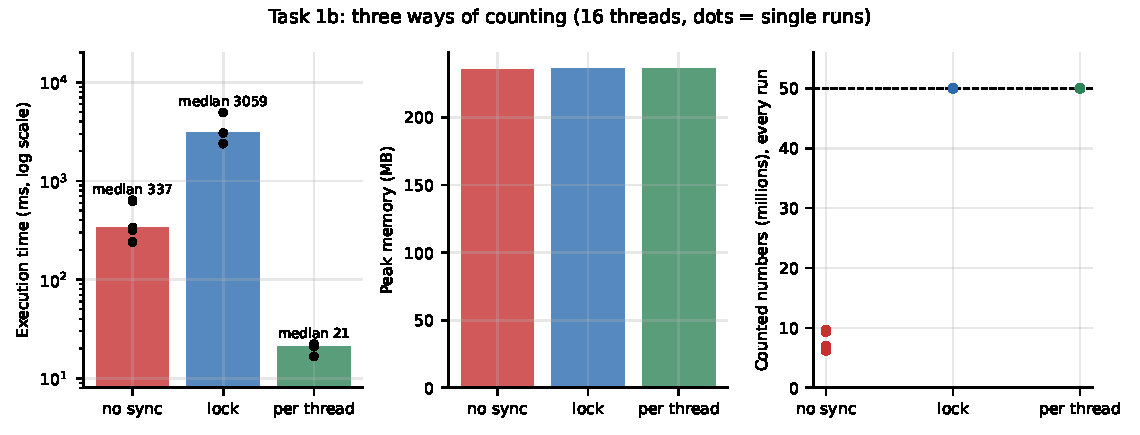
\includegraphics[width=\textwidth]{task1b.pdf}
\label{fig:task1b}
\end{figure}

\begin{table}[H]
  \centering
  \caption{Task 1b with \bThreads{} threads}
  \resizebox{\textwidth}{!}{\begin{tabular}{lrrrrr}
\toprule
Version & Runs & Median (ms) & Min--max (ms) & Peak mem. (MB) & Counted total \\
\midrule
1. no synchronisation & 9 & 337 & 239--636 & 236 & 6\,244\,509--9\,593\,146 \\
2. lock & 3 & 3059 & 2382--4939 & 236 & 50\,000\,000 \\
3. counter per thread & 3 & 21 & 17--22 & 236 & 50\,000\,000 \\
\bottomrule
\end{tabular}
}
  \label{tab:task1b}
\end{table}

\textbf{4. Rank the three versions by time. Which are correct? Explain each result.} The fastest is version 3, the counters of the threads: \bPerThreadMs{}~ms (\bPerThreadMsMin--\bPerThreadMsMax{}~ms in the three processes). Then comes version 1, without synchronisation: median \bNoSyncMs{}~ms, \bNoSyncRatio{} times slower than version 3, and its time changes much from run to run (\bNoSyncMsMin--\bNoSyncMsMax{}~ms). The slowest is version 2, the lock: median \bLockMs{}~ms (\bLockMsMin--\bLockMsMax{}~ms), \bLockRatio{} times slower than version 3. Only versions 2 and 3 are correct. Version 1 counted only \bNoSyncCountMin--\bNoSyncCountMax{} million of the 50 million numbers (at most \bNoSyncShareMax\%); a short time of a wrong program has no value.

\begin{itemize}
  \item \textit{Version 1.} The three counters lie next to each other, in one cache line, and 16 threads write into it all the time, so the processors must pass the line to each other after almost every increment; this is why even this version is much slower than version 3, and why its time depends on where the counters happen to lie in memory. The read--add--write sequences of different threads overlap, so most of the updates are lost.
  \item \textit{Version 2.} Every one of the 50 million updates takes the lock, so the counting is almost serial, and each acquisition also moves the lock and the counters between the processors and, under contention, puts the threads to sleep and wakes them.
  \item \textit{Version 3.} Each thread counts in its own variable, there is nothing shared, and only three additions per thread are made at the end. The time is limited by the reading of the array.
\end{itemize}

The peak memory is \bMemMin--\bMemMax{}~MB for all versions: it comes from the loading phase (the array alone has 190.7~MiB) and does not depend on the way of counting.

\subsection{Task 1c: Producer and Consumers}

Figure~\ref{fig:task1c} and Table~\ref{tab:task1c} show one reader and 1 to 64 workers, with a queue of 100 batches of 10\,000 lines.

\begin{figure}[H]
\centering
\caption{Task 1c: one reader, a variable number of workers}
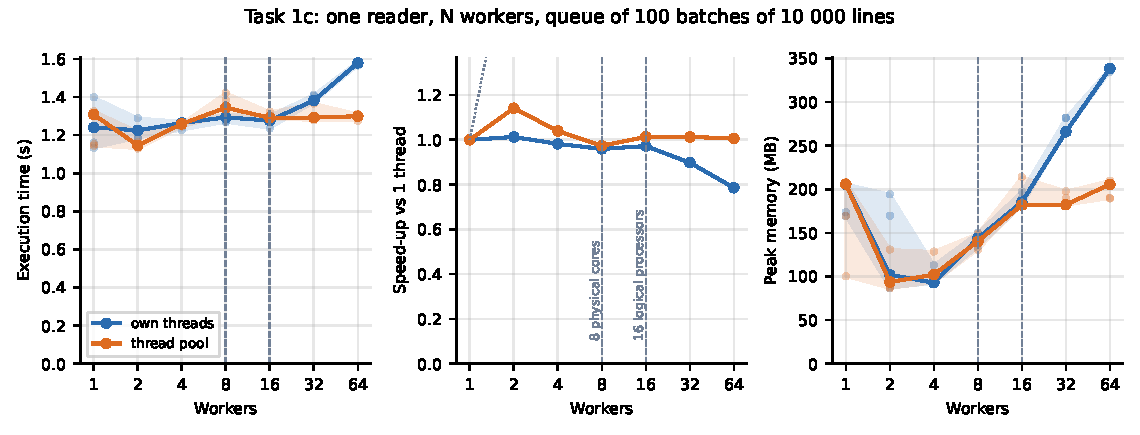
\includegraphics[width=\textwidth]{task1c.pdf}
\label{fig:task1c}
\end{figure}

\begin{table}[H]
  \centering
  \caption{Task 1c, median of \aRunsEach{} runs; the last three columns are the thread-pool variant}
  \resizebox{\textwidth}{!}{\begin{tabular}{rrrrrrr}
\toprule
Workers & Time (s) & Speed-up & Peak mem. (MB) & Pool: time (s) & Pool: speed-up & Pool: peak mem. (MB) \\
\midrule
1 & 1.241 & 1.00 & 205.7 & 1.308 & 1.00 & 205.8 \\
2 & 1.225 & 1.01 & 101.9 & 1.146 & 1.14 & 93.7 \\
4 & 1.264 & 0.98 & 92.8 & 1.259 & 1.04 & 102.1 \\
8 & 1.293 & 0.96 & 143.8 & 1.344 & 0.97 & 140.3 \\
16 & 1.276 & 0.97 & 185.2 & 1.291 & 1.01 & 182.0 \\
32 & 1.382 & 0.90 & 265.8 & 1.292 & 1.01 & 182.2 \\
64 & 1.579 & 0.79 & 338.5 & 1.299 & 1.01 & 205.6 \\
\bottomrule
\end{tabular}
}
  \label{tab:task1c}
\end{table}

\textbf{5. Compare Task 1c with Task 1a. Which is faster, and why? At which number of workers does Task 1c stop getting faster?} Task~1a is faster in every configuration: with one thread \aSecOne{}~s against \cSecOne{}~s for Task~1c (\cOverAOne{} times more), and the best results are \aSecBest{}~s and \cSecBest{}~s (\cOverABest{} times). In Task~1a all threads read and parse in parallel. In Task~1c the single reader must read 50 million lines, create a string for each of them and put the batches into the queue, and this sequential work takes about 1.2~s, which is the time of the whole program; the workers only parse short strings and wait for the reader most of the time. Therefore Task~1c does not get faster with more workers at all: one worker is already as fast as the reader (\cSecOne{}~s), the best result is with \cBestWorkers{} workers (\cSecBest{}~s, a speed-up of \cSpeedBest{}, which is within the variation of the runs with one worker, \cOneMin--\cOneMax{}~s), and with more workers it becomes slower: \cSlowdownSixtyFour\% with 64 workers (\cSecSixtyFour{}~s). The additional threads compete for the queue and cost memory (\cMemOne{}~MB with one worker, \cMemSixtyFour{}~MB with 64). With one worker the memory is the highest of the small values, probably because the reader is then faster than the worker and the queue fills up; with two or more workers the queue stays almost empty. We did not measure the occupancy of the queue.

\textbf{6. What would happen with batches of a single line? And with a queue that has no size limit?} With one line in a batch the program would need 50 million operations on the queue instead of 5\,000. Each of them takes a lock, may wake up a waiting thread and allocates a small list, so the cost of the synchronisation would be much larger than the cost of parsing a number; the program would become much slower, and more workers would make it worse because they would fight for the same lock. (We did not run this configuration; the batch size of the assignment is fixed in the program.) With a queue without a limit the reader never has to wait. In our program the workers keep up with the reader, so the queue would stay short and nothing would change. If the reader were faster than the workers, the queue would keep growing until it contained the whole file as strings; as an estimate, 50 million strings of about 40 bytes plus a reference of 8~bytes each are about 2.4~GB, much more than the 352~MiB file. The limit makes the reader wait and keeps the memory small.

\subsection{Task 1c with the Thread Pool}

In Task~1c the reader and the workers were also started with \texttt{Task.Run}. Up to 16 workers the two variants have similar times (within about 7\%, Table~\ref{tab:task1c}), but with 32 and 64 workers the pool is faster: \cPoolSecSixtyFour{}~s against \cSecSixtyFour{}~s with 64 workers (\cPoolGainSixtyFour\% less), and uses less memory (\cPoolMemSixtyFour{} against \cMemSixtyFour{}~MB). This is not a real speed-up. The workers wait for the queue, which means they block pool threads, and the pool starts only 16 threads at once, so with 64 workers only about 16 can be active at a time, as in the separate test of Section~\ref{sec:pool} (the others wait for a free thread and are not needed), whereas our 64 threads all fight for the queue and all hold memory. The pool therefore works here as a limit of the number of workers: the best result of the pool (\cPoolSecTwo{}~s with two workers) is not significantly better than the best result of our own threads (\cSecBest{}~s). The lecture rule ``never block a pool thread'' still applies: this program works only because the reader is started before the workers and the workers are not needed in the end; a pool full of waiting workers would delay a task that is started later.

\newpage
\section{Task 2: Many Files on Slow Storage}
\label{sec:task2}

The eight files were copied to the USB drive (USB~2.0, Table~\ref{tab:hardware}). The drive was ejected, unplugged and plugged in again before every run, so no data came from the page cache. Each configuration (1, 2 and 4 threads) was run three times, interleaved in the order 1, 2, 4, 1, 2, 4, 1, 2, 4; Figure~\ref{fig:task2} and Table~\ref{tab:task2} give the mean of the three runs. For comparison the same program was run on the internal SSD (the files had been read recently, so they were probably in the page cache; the result shows the cost of parsing and not of the disk).

\begin{figure}[H]
\centering
\caption{Task 2 on the USB drive: execution time, speed-up and peak memory}
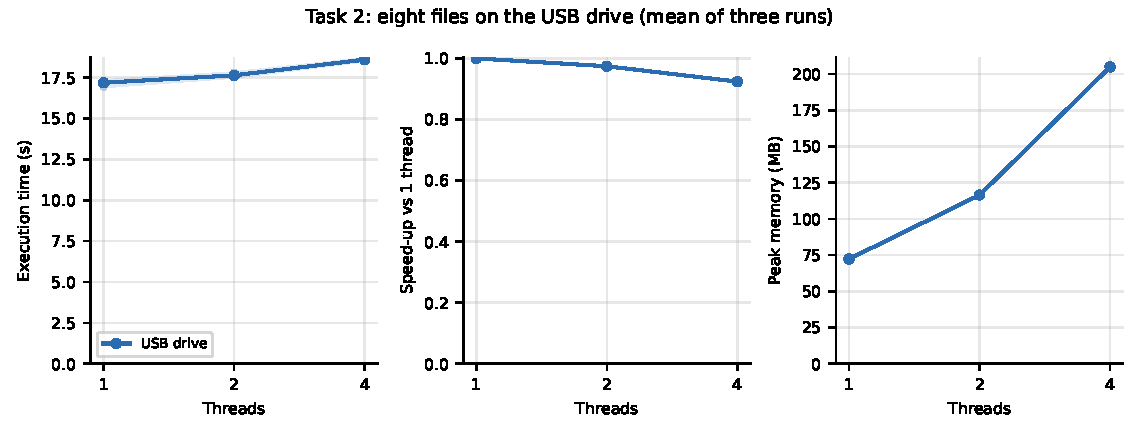
\includegraphics[width=\textwidth]{task2.pdf}
\label{fig:task2}
\end{figure}

\begin{table}[H]
  \centering
  \caption{Task 2: mean of three runs; reading and parsing are the times of all threads together}
  \resizebox{\textwidth}{!}{\begin{tabular}{lrrrrrrr}
\toprule
Storage & Threads & Time (s) & Speed-up & Reading (s) & Parsing (s) & Peak mem. (MB) & Runs \\
\midrule
USB drive & 1 & 17.19 & 1.00 & 16.43 & 0.75 & 72 & 3 \\
USB drive & 2 & 17.64 & 0.97 & 34.47 & 0.75 & 116 & 3 \\
USB drive & 4 & 18.60 & 0.92 & 71.88 & 0.74 & 205 & 3 \\
Internal SSD & 1 & 0.50 & 1.00 & 0.07 & 0.42 & 71 & 3 \\
Internal SSD & 2 & 0.28 & 1.78 & 0.06 & 0.49 & 115 & 3 \\
Internal SSD & 4 & 0.21 & 2.37 & 0.10 & 0.64 & 203 & 3 \\
\bottomrule
\end{tabular}
}
  \label{tab:task2}
\end{table}

\textbf{1. Compare one thread with Task 1a on one thread. Is the work CPU-bound or I/O-bound?} On the USB drive one thread needs \tUsbSecOne{}~s, against \aSecOne{}~s for Task~1a (\tUsbOverA{} times more) and \tSsdMsOne{}~ms for the same program on the internal SSD (\tUsbOverSsd{} times less). The parsing is a small part of the time in both cases (\tUsbParseOne{}~s on the USB drive, \tSsdParseOne{}~s on the SSD), but the reading takes \tUsbReadOne{}~s on the USB drive and only \tSsdReadOne{}~s on the SSD (Figure~\ref{fig:task2b}). On the USB drive \tUsbReadShare\% of the time is reading: a read speed of about \tUsbMiBs{}~MiB/s, normal for a USB~2.0 flash drive. The work is therefore \textbf{I/O-bound} on the USB drive. On the SSD, in Task~1a and in all other tasks it is CPU-bound, with only \tSsdReadShare\% of the time in reading.

\begin{figure}[H]
\centering
\caption{Task 2: reading and parsing time (log scale)}
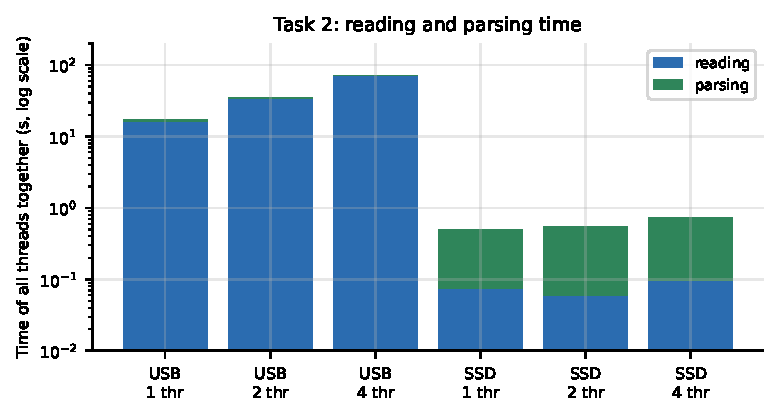
\includegraphics[width=0.62\textwidth]{task2-breakdown.pdf}
\label{fig:task2b}
\end{figure}

\textbf{2. Do more threads help on the USB drive? Why not, when lecture 1 showed that I/O-bound work benefits from concurrency?} No. The time is \tUsbSecOne{}~s with one thread, \tUsbSecTwo{}~s with two (speed-up \tUsbSpeedTwo) and \tUsbSecFour{}~s with four (\tUsbSpeedFour); the three runs of one configuration differ by less than 0.5~s, so the line is flat and, if anything, a little worse with more threads. The reading time of all threads together doubles and quadruples (\tUsbReadOne{}, \tUsbReadTwo{} and \tUsbReadFour{}~s), because the threads wait for each other: all of them read through one USB~2.0 link from one flash drive, so each of them receives a smaller share of the same bandwidth. A separate test confirms this (\texttt{dd} with direct I/O, which bypasses the cache, three repetitions, \texttt{data/usb-throughput.txt}): one reader gets 23.2~MiB/s, two readers 21--22~MiB/s together and four readers 20.6~MiB/s together. Concurrency helps an I/O-bound program when the waits are independent and the device has free capacity, as with a server that waits for many different clients, each answering in its own time; here there is one shared device that one thread already uses completely. On the SSD, where the work is mostly parsing, more threads do help (\tSsdSpeedTwo{} with two and \tSsdSpeedFour{} with four threads). More threads cost memory in Task~2: each thread holds a buffer for a whole file of about 46~MB, so the peak is \tUsbMemOne{}, \tUsbMemTwo{} and \tUsbMemFour{}~MB.

\newpage
\section{Control Questions}

\subsection{Physical Core and Logical Processor}

A physical core is a complete computing unit; a logical processor is a hardware thread that the operating system can schedule, and with hyper-threading one core shows two of them that share its execution units. This processor has 8 cores and 16 logical processors. In our charts it is the place of the dashed lines in Figures~\ref{fig:task1a} and~\ref{fig:task1c}: in Task~1a the speed-up grows almost linearly up to 8 threads (\aSpeedEight) and does not grow between 8 and 16 threads (\aSpeedSixteen) and further.

\subsection{No Line Counted Twice or Skipped}

The rough cut at $\mathit{size}\cdot i/N$ is moved to the first byte after the next newline, searching from the byte before the cut, so a line that starts exactly at the cut is not lost. The range of a thread is from its start to the start of the next thread, and both are computed by the same function, so each line belongs to exactly one thread. All runs of Task~1a, with every number of threads from 1 to 64, gave exactly the counters of the generator.

\subsection{Why Unsynchronised Shared Counters Lose Updates}

Suppose the counter holds 10 and two threads add one. (1)~Thread A reads 10. (2)~Thread B reads 10. (3)~A computes 11. (4)~B computes 11. (5)~A writes 11. (6)~B writes 11. Two increments were made, but the counter grew by one. With 16 threads this happens all the time: in our runs only \bNoSyncCountMin--\bNoSyncCountMax{} million of the 50 million updates remained.

\subsection{Why Counters of the Threads Are Faster Than a Lock}

A lock makes the 50 million updates run one after another, and every acquisition costs time even when nobody waits, because the lock and the counters move between the caches of the processors; under contention the threads are also put to sleep and woken. With a counter for each thread nothing is shared while counting, and the synchronisation is reduced from one per number to one per thread: \bPerThreadMs{}~ms against \bLockMs{}~ms in our runs.

\subsection{I/O-bound for a USB Drive and for a Network Server}

For a USB drive ``I/O-bound'' means that the time is spent waiting until the device delivers the data: in Task~2 \tUsbReadShare\% of the time was reading at about \tUsbMiBs{}~MiB/s. For a server waiting for the network the time is spent waiting for the other side. Concurrency helps in the network case because the waits belong to different, independent clients: while one request waits for its answer, the processor serves another, and the throughput grows. The USB drive is one device with one limited bandwidth, which one thread already uses completely, so more threads only wait for the same resource, as Task~2 showed.

\subsection{Equal Parts in Advance or a Queue}
\label{cq:queue}

Dividing the work in advance (Task~1a) costs nothing while the program runs: there is no shared structure and no lock, and every thread reads its own contiguous part. It is better when the parts need about the same time, as here. A queue (Task~1c) gives the next piece to the worker that is free, so it balances parts of unequal cost, and it allows one producer to feed the workers when the data cannot be divided in advance (a stream, a network). The price is the lock of the queue, the batches in memory and a sequential producer, which in our case decided the time of the whole program: \cSecBest{}~s against \aSecBest{}~s for the division in advance.

\newpage
\section{Conclusions}

The measurements on this machine (8 physical cores, 16 logical processors) show that the structure of the work matters more than the number of threads. Counting one file in independent, line-aligned parts (Task~1a) is CPU-bound: the speed-up is almost linear up to four threads, reaches \aSpeedEight{} with the 8 physical cores and does not grow with 16, 32 and 64 threads, while the memory grows by about 1~MiB for every thread. Threads from the thread pool gave the same times as our own threads, because the work is long compared with the cost of creating a thread.

On the shared array the two correct versions differ much: the counters of the threads need \bPerThreadMs{}~ms and the lock \bLockMs{}~ms. Without synchronisation the program loses more than 80\% of the updates and the result is wrong; its time varies from \bNoSyncMsMin{} to \bNoSyncMsMax{}~ms because the threads share a cache line. The producer--consumer version (Task~1c) was \cOverABest{} times slower than the independent parts, because one reader reads and builds the strings of 50 million lines; more workers did not help, and with 64 own threads the program became \cSlowdownSixtyFour\% slower. The thread pool avoided this only because it runs at most 16 threads at once.

Task~2 was I/O-bound: with the files on a USB~2.0 flash drive \tUsbReadShare\% of the time was spent reading at about \tUsbMiBs{}~MiB/s, the run took \tUsbOverA{} times longer than Task~1a, and extra threads gave no speed-up (\tUsbSpeedTwo{} and \tUsbSpeedFour) because all of them waited for the same drive. In short, on this machine Tasks~1a, 1b and Task~2 on the SSD were CPU-bound, Task~1c was limited by its single reader, and Task~2 on the USB drive was I/O-bound. The results are limited by \aRunsEach{} runs for Tasks~1a and~1c, three runs for Task~2, and by the other programs that ran on the laptop; the conclusions concern differences that are large compared with this variation.

\section{Source Code}

The C\# source code, the csv files with all measurements and this report are available in the repository:

\begin{center}
  \url{https://github.com/Moisei-D/PR-Labs}
\end{center}

The program is in the folder \texttt{Lab1} (one file for every task) and the report in \texttt{Reports/Lab1 Report}. The \texttt{README.md} of the project lists all commands; for example:

\begin{terminaloutput}
cd Lab1
dotnet build -c Release
dotnet run -c Release -- generate
dotnet run -c Release -- split
dotnet run -c Release -- task1a --threads 8
dotnet run -c Release -- task1a --threads 8 --pool
dotnet run -c Release -- task1b
dotnet run -c Release -- task1c --threads 8
dotnet run -c Release -- task2 --dir /path/to/usb --threads 2 --storage usb
\end{terminaloutput}

\end{document}
